\documentclass[tikz,border=10pt]{standalone}
\usepackage[T1]{fontenc}
\usepackage[utf8]{inputenc}
\usepackage{libertine}
\usepackage{graphicx}
\usepackage{amsmath,amssymb}
\usepackage{xcolor}
\usetikzlibrary{arrows.meta,positioning,backgrounds,shapes.geometric,
                calc,fit,decorations.pathreplacing}

\begin{document}

\tikzset{
  ovImg/.style  = {inner sep=0pt, outer sep=0pt},
  ovFm/.style   = {inner sep=0pt, outer sep=0pt},
  ovStem/.style = {draw=gray!70, fill=cyan!10, rounded corners=3pt,
                   minimum width=2.0cm, minimum height=0.62cm,
                   align=center, line width=0.8pt},
  ovEnc/.style  = {draw=blue!60!black, fill=blue!10, rounded corners=3pt,
                   minimum width=2.3cm, minimum height=0.62cm,
                   align=center, line width=0.8pt},
  ovBot/.style  = {draw=teal!70!black, fill=teal!12, rounded corners=3pt,
                   minimum width=2.3cm, minimum height=0.62cm,
                   align=center, line width=1.0pt},
  ovVae/.style  = {draw=purple!65!black, fill=purple!8, rounded corners=3pt,
                   minimum width=3.2cm, minimum height=0.72cm,
                   align=center, line width=1.0pt, dashed},
  ovDec/.style  = {draw=orange!65!black, fill=orange!10, rounded corners=3pt,
                   minimum width=2.3cm, minimum height=0.62cm,
                   align=center, line width=0.8pt},
  ovHead/.style = {draw=teal!60!black, fill=teal!9, rounded corners=3pt,
                   minimum width=2.0cm, minimum height=0.62cm,
                   align=center, line width=0.8pt},
  ovMc/.style   = {draw=purple!55!black, fill=purple!7, rounded corners=3pt,
                   minimum width=2.2cm, minimum height=0.55cm,
                   align=center, line width=0.8pt, dashed},
  ovDim/.style  = {font=\fontsize{7}{8}\selectfont, text=black!60, align=center},
  ovMain/.style = {->, line width=1.3pt, black!70},
  ovSkip/.style = {->, line width=1.1pt, blue!65, dashed},
  ovByp/.style  = {->, line width=0.9pt, gray!60, dashed},
  ovVaeA/.style = {->, line width=1.0pt, purple!65},
}

% RULE: \\ must appear at the TOP LEVEL of node content only.
% Never place \\ inside a {group} — newer LaTeX injects \scan_stop: there.

\begin{tikzpicture}[>=Stealth, every node/.style={font=\small}]

% ── Input ────────────────────────────────────────────────────────────
\node[ovImg] (inp) at (-2.5,11.0)
  {\includegraphics[width=1.3cm,height=1.3cm,keepaspectratio]%
    {figures/arch/arch_input_noisy.png}};
\node[ovDim] at (-2.5,12.0)
  {Noisy CXR\\[-2pt]$1{\times}256{\times}256$};

% ── Encoder (left column) ────────────────────────────────────────────
\node[ovStem] (stem) at (-2.5,9.6)
  {\textbf{Stem}\\
   {\fontsize{6}{7}\selectfont Conv $3{\times}3$, $1{\to}64$\,ch}};

\node[ovEnc] (enc1) at (-2.5,8.1)
  {\textbf{E1}\\
   {\fontsize{6}{7}\selectfont HB${\times}2$+Down,\;64\,ch,\;$256^2$}};

\node[ovEnc] (enc2) at (-2.5,6.5)
  {\textbf{E2}\\
   {\fontsize{6}{7}\selectfont HB${\times}2$+Down,\;128\,ch,\;$128^2$}};

\node[ovEnc] (enc3) at (-2.5,4.9)
  {\textbf{E3}\\
   {\fontsize{6}{7}\selectfont HB${\times}2$+Down,\;256\,ch,\;$64^2$}};

\node[ovBot] (bot) at (-2.5,3.3)
  {\textbf{Bottleneck}\\
   {\fontsize{6}{7}\selectfont HB${\times}2$,\;$512$\,ch,\;$32^2$}};

% ── VAE branch ───────────────────────────────────────────────────────
\node[ovVae] (vae) at (0,1.9)
  {\textbf{VAE Bottleneck}\\
   {\fontsize{6}{7}\selectfont $z{=}\mu_z{+}\varepsilon\!\cdot\!\exp(\tfrac{1}{2}\sigma_z^2)$}};

\node[ovMc] (mc) at (0,0.6)
  {{\fontsize{6}{7}\selectfont $K{=}20$ stochastic passes}};

% ── Decoder (right column) ───────────────────────────────────────────
\node[ovDec] (dec3) at (2.5,4.9)
  {\textbf{D3}\\
   {\fontsize{6}{7}\selectfont Up+$s_3$+HB${\times}2$,\;$64^2$}};

\node[ovDec] (dec2) at (2.5,6.5)
  {\textbf{D2}\\
   {\fontsize{6}{7}\selectfont Up+$s_2$+HB${\times}2$,\;$128^2$}};

\node[ovDec] (dec1) at (2.5,8.1)
  {\textbf{D1}\\
   {\fontsize{6}{7}\selectfont Up+$s_1$+HB${\times}2$,\;$256^2$}};

\node[ovHead] (head) at (2.5,9.6)
  {\textbf{Dual Head}\\
   {\fontsize{6}{7}\selectfont Conv\,$3{\times}3$}};

% ── Output thumbnails ────────────────────────────────────────────────
% All three outputs are Arm H inference on the same arch_input_noisy.png patient.
\node[ovImg] (outmu) at (4.5,10.2)
  {\includegraphics[width=1.1cm,height=1.1cm,keepaspectratio]%
    {figures/arch/arch_output_mu.png}};
\node[ovDim, above=2pt of outmu] {$\hat{\mu}_y$};

\node[ovImg] (outsig) at (4.5,9.0)
  {\includegraphics[width=1.1cm,height=1.1cm,keepaspectratio]%
    {figures/arch/arch_output_aleat.png}};
\node[ovDim, below=2pt of outsig] {$\hat{\sigma}^2_a$};

\node[ovImg] (outepi) at (2.5,0.6)
  {\includegraphics[width=1.0cm,height=1.0cm,keepaspectratio]%
    {figures/arch/arch_output_epist.png}};
\node[ovDim, right=3pt of outepi] {$\hat{\sigma}^2_e$};

% ── Skip FM icons ─────────────────────────────────────────────────────
\node[ovFm] (fm_s1) at (0,8.1)
  {
\includegraphics[width=0.45cm,height=0.45cm]{figures/arch/featmap_256.png}};
\node[ovDim, above=1pt of fm_s1] {$s_1$};

\node[ovFm] (fm_s2) at (0,6.5)
  {
\includegraphics[width=0.40cm,height=0.40cm]{figures/arch/featmap_128.png}};
\node[ovDim, above=1pt of fm_s2] {$s_2$};

\node[ovFm] (fm_s3) at (0,4.9)
  {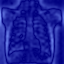
\includegraphics[width=0.34cm,height=0.34cm]{figures/arch/featmap_64.png}};
\node[ovDim, above=1pt of fm_s3] {$s_3$};

% ── Main flow arrows ──────────────────────────────────────────────────
\draw[ovMain] (inp.south)  -- (stem.north);
\draw[ovMain] (stem.south) -- (enc1.north);
\draw[ovMain] (enc1.south) -- (enc2.north);
\draw[ovMain] (enc2.south) -- (enc3.north);
\draw[ovMain] (enc3.south) -- (bot.north);

% bot → VAE → dec3  (main probabilistic path)
\draw[ovMain] (bot.south) |- (vae.west);
\draw[ovMain] (vae.east)  -| (dec3.south);

% bot → dec3 bypass (Arms A–D, no VAE)
\draw[ovByp] (bot.east) -|
  node[above, pos=0.22,
       font=\fontsize{6}{7}\selectfont, text=gray!60]
    {Arms\,A--D}
  (dec3.south);

\draw[ovMain] (dec3.north) -- (dec2.south);
\draw[ovMain] (dec2.north) -- (dec1.south);
\draw[ovMain] (dec1.north) -- (head.south);

% head → outputs (fork: shared stem drawn once, then two branches)
\coordinate (headBr) at ($(head.east)+(0.45,0)$);
\draw[ovMain] (head.east) -- (headBr) -- ++(0, 0.6) -- (outmu.west);
\draw[ovMain] (headBr)    --            ++(0,-0.6) -- (outsig.west);

% VAE → MC → epistemic output
\draw[ovVaeA] (vae.south) -- (mc.north);
\draw[ovVaeA] (mc.east)   -- (outepi.west);

% Skip connections (encoder → FM icon → decoder)
\draw[ovSkip] (enc1.east)  -- (fm_s1.west);
\draw[ovSkip] (fm_s1.east) -- (dec1.west);
\draw[ovSkip] (enc2.east)  -- (fm_s2.west);
\draw[ovSkip] (fm_s2.east) -- (dec2.west);
\draw[ovSkip] (enc3.east)  -- (fm_s3.west);
\draw[ovSkip] (fm_s3.east) -- (dec3.west);

\end{tikzpicture}

\end{document}
